\section{Essaim de robots reconfigurables et modulaires}
\label{essaim_de_drones}

Cette section traite des systèmes d'essaims de robots et de drones reconfigurables. Un état de l’art détaillé sur le projet eSWARM a été réalisé en 2024 par Augustin Bonnel \cite{bonnel_modeling_2024}. En raison de la pertinence de son analyse, certains travaux et articles décrits dans son rapport seront repris ici, car ils constituent une base solide. Toutefois, des compléments et mises à jour seront apportés, puisque de nouveaux documents ont été publiés depuis.

\subsection{Exemples de systèmes modulaires}

Parmi les systèmes modulaires, il est possible de définir deux catégories : les systèmes autonomes et non autonomes. Dans la seconde catégorie, le système doit être composé d'un nombre minimum de modules pour pouvoir fonctionner, contrairement à la première. Le système final visé dans le projet eSWARM est donc autonome, puisqu'il est constitué de quadcoptères indépendants.

\subsubsection*{Systèmes non autonomes}

\begin{wrapfigure}{r}{0.5\textwidth}
    \vspace{-0.2cm} 
    \centering
    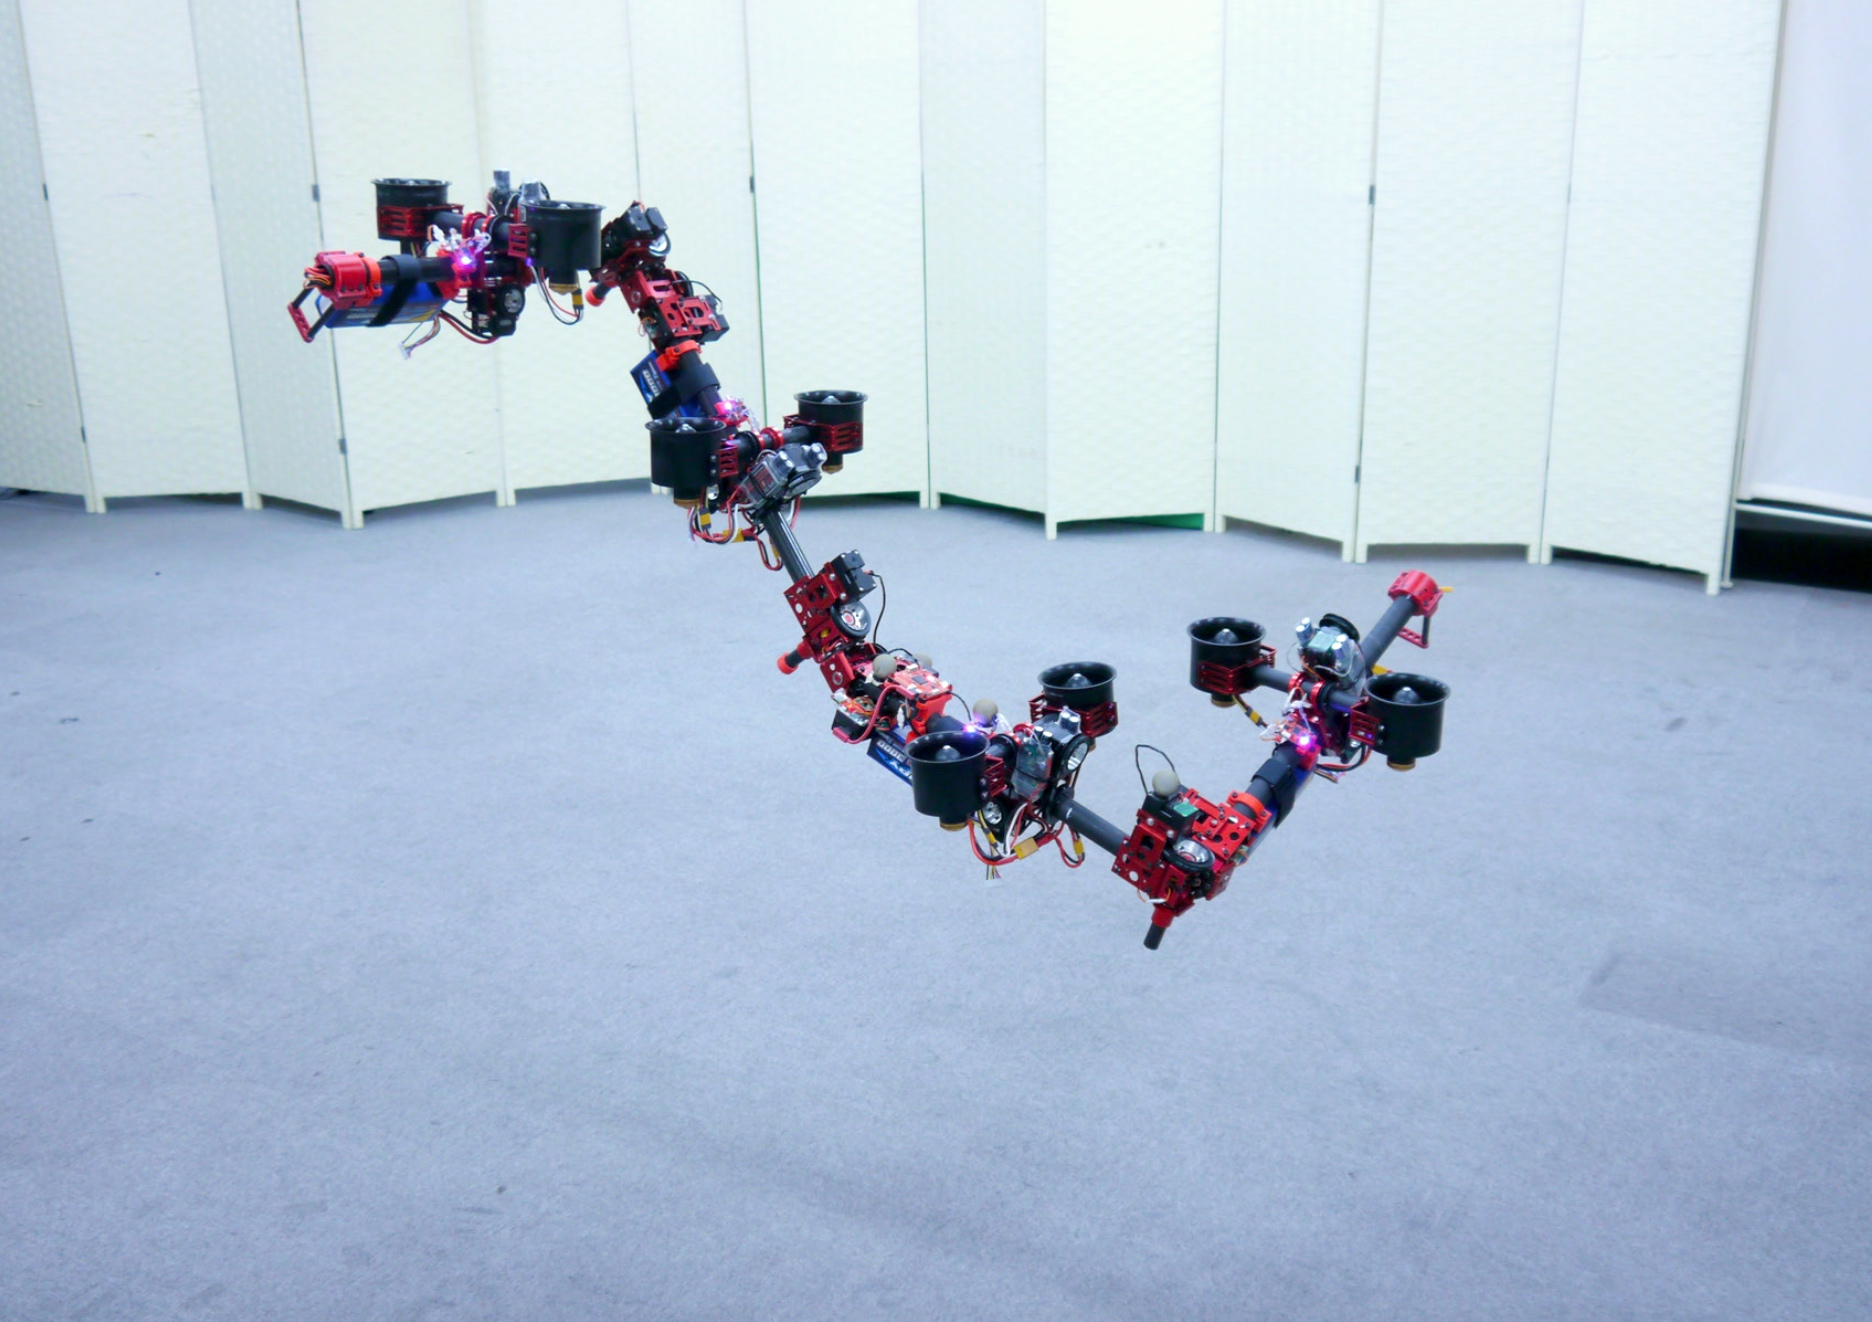
\includegraphics[scale=0.13]{8-Etat_de_art/eswarm/pic/dragon-drone.jpeg}
    \caption{Drone DRAGON \protect\cite{zhao_design_2018}}
    \label{fig:dragon}
    \vspace{-0.3cm} 
\end{wrapfigure}

Le DRAGON Drone ("Dual-rotor embedded multilink Robot with the Ability of multi-degree of freedom") \cite{zhao_design_2018} est un projet non autonome. Ce système modulaire, développé par l'Université de Tokyo, est inspiré du mouvement des dragons chinois. Il est constitué de plusieurs modules reliés par des articulations motorisées, ce qui lui permet de modifier sa forme en vol et ainsi de se faufiler dans des espaces restreints ou de contourner des obstacles. Chaque module est équipé de ses propres rotors, et l’ensemble est contrôlé de manière coordonnée. Il partage donc certains objectifs du projet eSWARM. Une vidéo du projet est disponible \href{https://www.youtube.com/watch?v=vxsAKi_g1jA}{\underline{ici}}.

D'autres systèmes non autonomes existent, tels que ceux décrits dans \cite{garanger_modeling_2020} et \cite{schiano_reconfigurable_2022}, bien qu'ils s'éloignent des objectifs d'eSWARM. Le premier document présente un système de tetracoptère, composé de plusieurs modules uni-rotor pouvant s'assembler. Le second document évoque un drone cargo modulaire où le colis devient la structure centrale, avec des modules de propulsion attachés selon sa masse et sa forme. Contrairement au drone DRAGON, ces deux systèmes ne peuvent pas se réorganiser en vol ; leur configuration doit être définie à l'avance, ce qui signifie qu'ils ne sont pas véritablement reconfigurables.

Il convient de noter que la plupart des systèmes aériens non autonomes sont constitués de modules uni-rotors ou bi-rotors.


\subsubsection*{Systèmes autonomes}

Les systèmes se rapprochant le plus du projet eSWARM sont les projets ModQuad \cite{saldana_modquad_2018} et ModQuad-DoF \cite{gabrich_modquad-dof_2020} (voir Fig. \ref{fig:Modquad} et Fig.\ref{fig:Modquad-DoF}). Il s'agit dans les deux cas de drones quadcoptères CrazyFlie (identiques à ceux utilisés par le passé pour le projet eSWARM  \cite{bonnel_modeling_2024,boegeat_rapport_2023}) modifiés, afin de pouvoir s'accrocher ou non en l'air, et ainsi former une structure de plusieurs quadcoptères. ModQuad-DoF (2020) correspond à une autre version du ModQuad (2018), avec un système d'accroche est modifié permettant un degrés de liberté entre les drones. 

Les modèles de ces deux systèmes servent de référence pour le projet eSWARM et seront détaillés dans la partie \ref{part:control}. Ces projets appartiennent à la catégorie des systèmes modulaires reconfigurables.

\begin{figure}[htbp]
    \centering
    \begin{minipage}[b]{0.48\textwidth}
        \centering
        
\includegraphics[height=3.6cm]{8-Etat_de_art/eswarm/pic/modquad.png}
        \caption{ModQuad \protect\cite{saldana_modquad_2018}}
        \label{fig:Modquad}
        \vspace{-0.4cm}
    \end{minipage}
    \hfill
    \begin{minipage}[b]{0.48\textwidth}
        \centering
        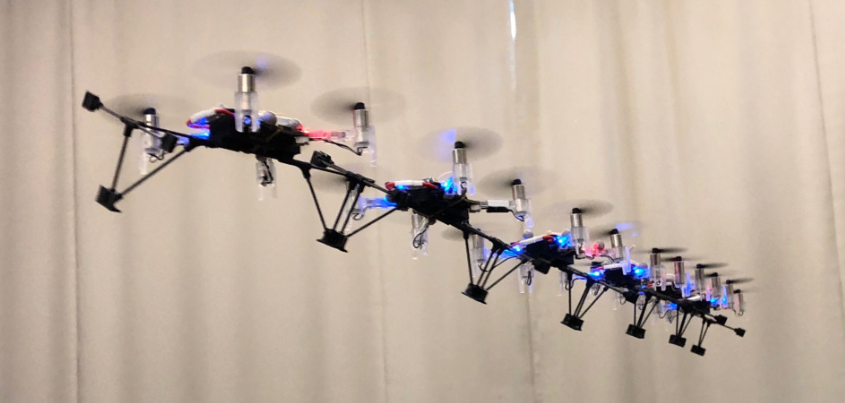
\includegraphics[height=3.6cm]{8-Etat_de_art/eswarm/pic/modquad_dof.PNG}
        \caption{ModQuad-DoF \protect\cite{gabrich_modquad-dof_2020}}
        \label{fig:Modquad-DoF}
        \vspace{-0.4cm}
    \end{minipage}
\end{figure}
Bien que les ModQuads puissent s'assembler en vol (voir vidéo \href{https://www.youtube.com/watch?v=25zKLyOCA3A&t=80s}{\underline{ici}}), le système rencontre encore des difficultés lors du désassemblage. Les forces magnétiques utilisées semblent trop puissantes pour un détachement fluide, comme mentionné dans \cite{sugihara_beatle_2024}, qui propose un mécanisme combinant aimants et connecteurs mécaniques.

\cite{zhang_design_2024} décrit un projet similaire à eSWARM, l’un des plus récents à ce jour. Les drones utilisés sont des quadcoptères modifiés dont les rotors peuvent pivoter, ajoutant des degrés de liberté. Cette caractéristique permet de générer des forces directionnelles facilitant la séparation des modules tout en maintenant l'alignement des structures d'accroche. Une démonstration vidéo est disponible \href{https://www.youtube.com/watch?v=EtJYZaVobcI}{\underline{ici}}. Ainsi, les modules se séparent en douceur, évitant les déséquilibres et conservant leur stabilité. De plus, des électro-aimants, accompagnés d'un système mécanique sont utilisés pour accrocher deux modules, ce qui permet de piloter le système d'accroche avec un programme. 

\begin{figure}[H]
    \centering
        \vspace{-0.1cm}  % Ajustez cette valeur pour réduire l'espace
    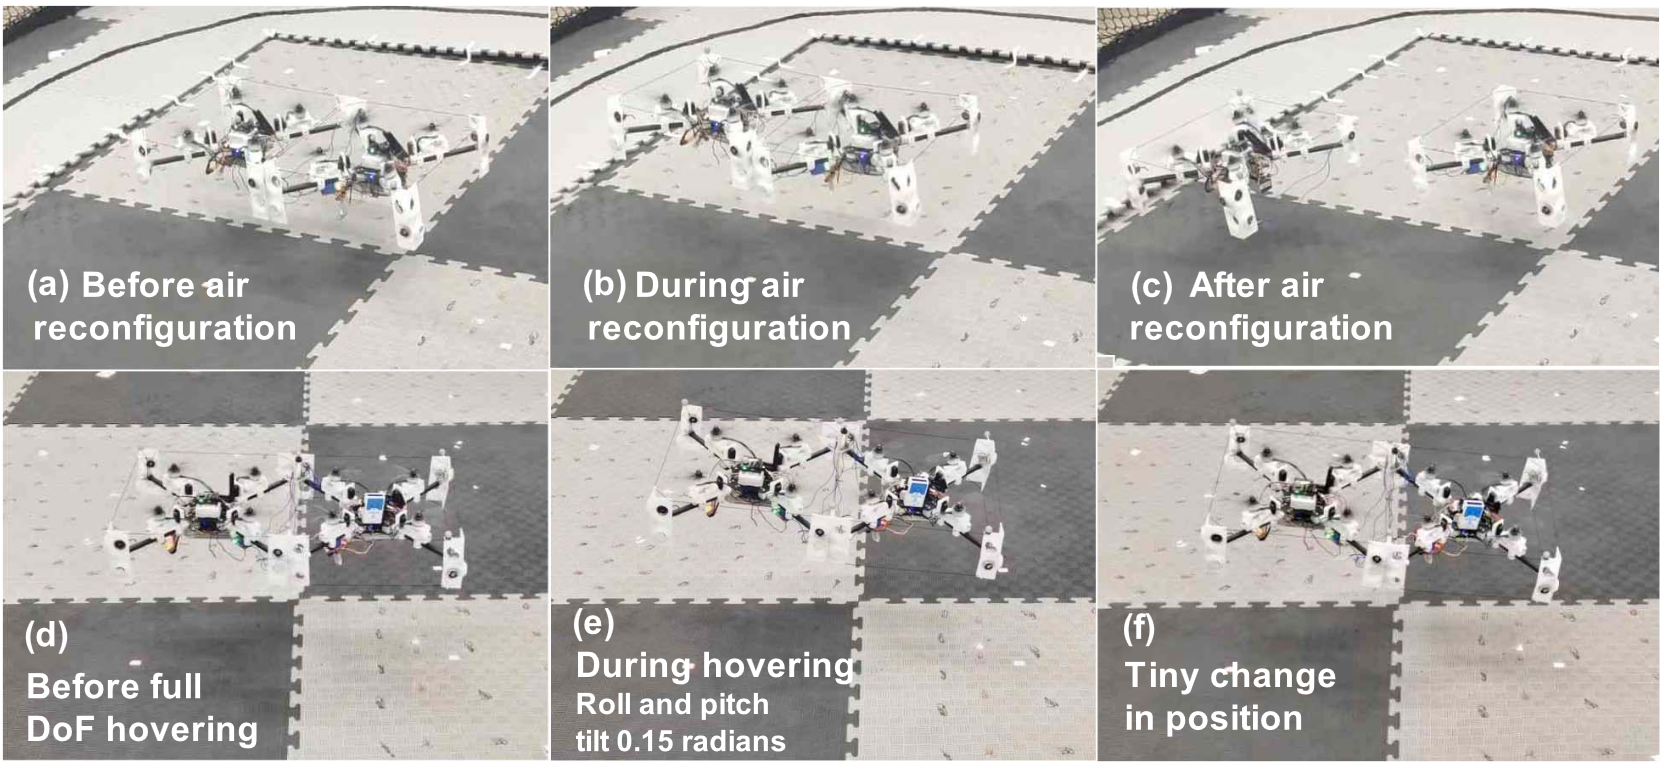
\includegraphics[scale=0.3]{8-Etat_de_art/eswarm/pic/assemblage.PNG}
    \vspace{-0.2cm}  % Ajustez cette valeur pour réduire l'espace
    \caption{Désassemblage en vol du système \protect\cite{zhang_design_2024}}
    \label{fig:assemblage}
        \vspace{-0.4cm}  % Ajustez cette valeur pour réduire l'espace
\end{figure}

Le laboratoire DRAGON, situé à Tokyo, à l'origine du système Figure \ref{fig:dragon}, a aussi travaillé sur plusieurs versions de système modulaires reconfigurables autonomes : 
\begin{itemize}
    \item TRADY \cite{junichiro_workshop_2025,sugihara_design_2023}: Le système d'accroche de TRADY combine des aimants permanents à commutation magnétique (pour un couplage/découplage rapide) et des ergots mobiles verrouillables, permettant à la fois une connexion rigide pour les manipulations et une tolérance aux erreurs de positionnement lors de l'assemblage en vol.
    \item BEATLE \cite{junichiro_workshop_2025,sugihara_beatle_2024} : chaque drone est contrôlé en position tout au long du vol, que le système soit en configuration assemblée ou désassemblée. Lorsqu'il est assemblé, les positions souhaitées des modules sont calculées en fonction de la position et de l'orientation souhaitées de la structure.
    \item LEGION \cite{junichiro_workshop_2025} : système constitué de tri-coptères
\end{itemize}

\begin{figure}[htbp]
    \centering
    \begin{minipage}[b]{0.48\textwidth}
        \centering
        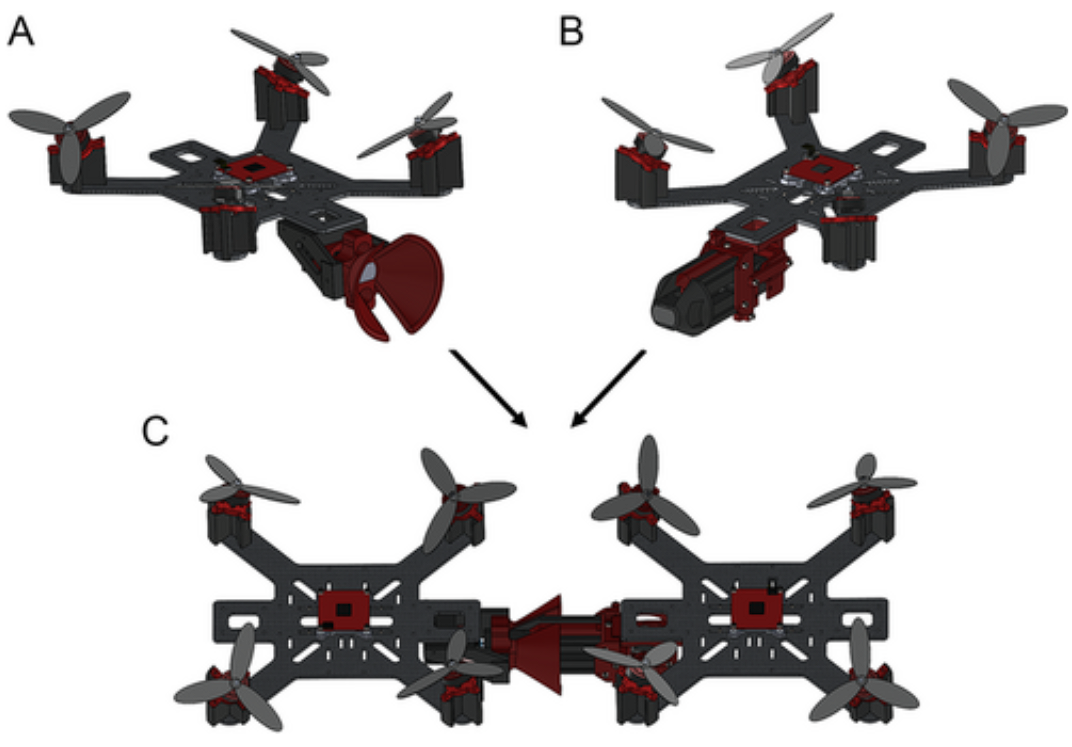
\includegraphics[height=3.6cm]{8-Etat_de_art/eswarm/pic/trady.png}
        \caption{Système TRADY \protect\cite{sugihara_design_2023}}
        \label{fig:trady}
    \end{minipage}
    \hfill
    \begin{minipage}[b]{0.48\textwidth}
        \centering
        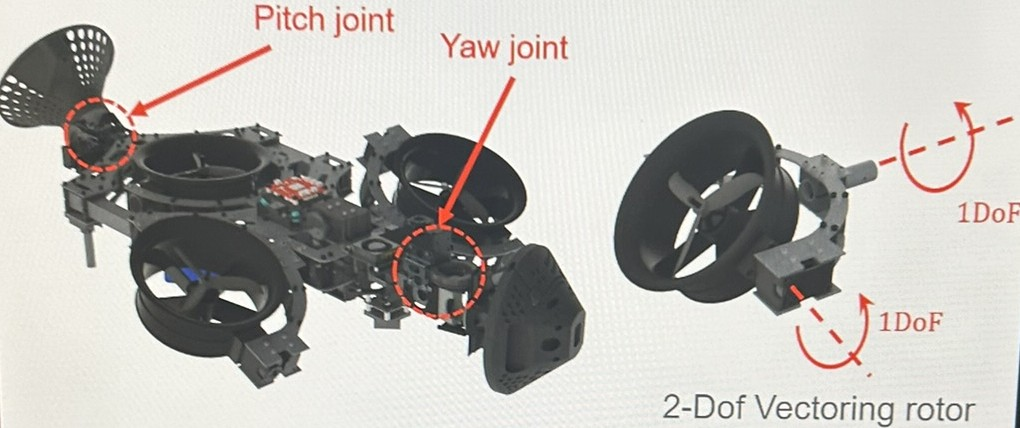
\includegraphics[height=3.6cm]{8-Etat_de_art/eswarm/pic/LEGION.JPEG}
        \caption{Système LEGION \protect\cite{junichiro_workshop_2025}}
        \label{fig:kegion}
    \end{minipage}
\end{figure}

\begin{figure}[H]
    \centering
        \vspace{-0.1cm}  % Ajustez cette valeur pour réduire l'espace
    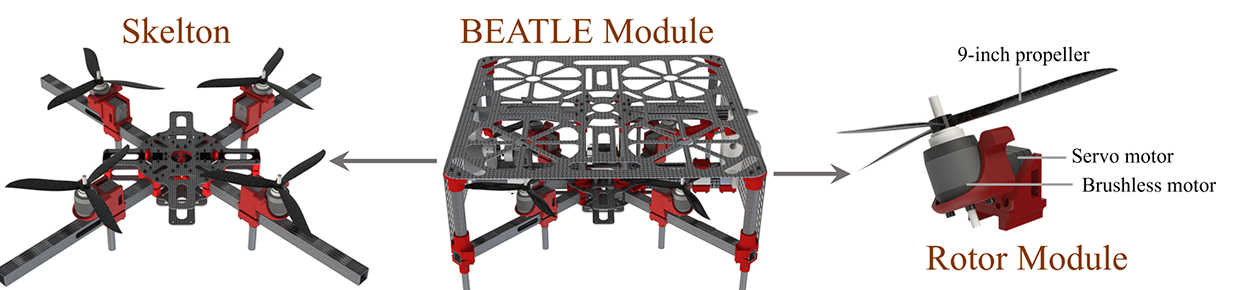
\includegraphics[scale=0.5]{8-Etat_de_art/eswarm/pic/beatle.png}
    \vspace{-0.2cm}  % Ajustez cette valeur pour réduire l'espace
    \caption{Système BEATLE \protect\cite{sugihara_beatle_2024}}
    \label{fig:BEATLE}
        \vspace{-0.4cm}  % Ajustez cette valeur pour réduire l'espace
\end{figure}

Les structures d'accroche des différents systèmes décrits ici sont plus robustes et complexes que celui développé dans le cadre de eSWARM, qui est donc éventuellement à revoir.

\subsection{Modélisation d'un système de drone modulaire}
\label{part:control}

%\noindent{Le modèle d'un unique quadcoptère est donné en annexe} \ref{modelisation_quadcopter}, sur la base de \cite{bonnel_modeling_2024} et \cite{gangloff_mooc_2023}, et sert de base pour la modélisation du système eSWARM et des autres projets qui s'en rapprochent.

\subsubsection*{Modélisation}

\noindent La modélisation décrite ici est basée sur \cite{bonnel_modeling_2024, saldana_modquad_2018}.

\noindent Les hypothèses sont les suivantes :

\begin{itemize}
    \item Le modèle du système varie selon la configuration de la structure, une occurrence du modèle est calculée chaque fois que la structure change. 
    \item Tous les modules partagent la même orientation, l'angle de lacet de tous les modules et de la structure entière est considéré comme nul.
    \item Tous les modules connaissent leur position et orientation dans le repère monde.
    \item Tous les modules sont symétriques, par conséquent la matrice d'inertie d'un module est diagonale.
\end{itemize}

%D'après le modèle d'un quadcoptère (annexe \ref{modelisation_quadcopter}, la force et les moments exercés par une hélice sur celle-ci sont proportionnels au carré de la vitesse angulaire de cette hélice. Or, comme le centre de masse dépend du nombre de modules et de leur configuration, le torseur de la structure dépend des mêmes paramètres. Le torseur de la structure est :

\[
\begin{bmatrix}F\\ M_{x}\\ M_{y}\\ M_{z}\end{bmatrix}=\sum_{i}\begin{bmatrix}1&1&1&1\\ y_{i1}&y_{i2}&y_{i3}&y_{i3}\\ -x_{i1}&-x_{i2}&-x_{i3}&-x_{i4}\\ \frac{k_{M}}{k_{F}}&\frac{k_{M}}{k_{F}}&\frac{k_{M}}{k_{F}}&\frac{k_{M}}{k_{F}} \\ \end{bmatrix}\begin{bmatrix}f_{i1}\\ f_{i2}\\ f_{i3}\\ f_{i4}\end{bmatrix}
\]
où \(\begin{bmatrix}F&M_{x}&M_{y}&M_{z}\end{bmatrix}^{T}\) représentent respectivement la poussée, les moments de tangage, de roulis et de lacet de la structure, \(f_{ij}\) est la force générée par une hélice, \((x_{ij},y_{ij})\) la distance de la \(j^{\text{ème}}\) hélice du \(i^{\text{ème}}\) module par rapport au centre de masse de la structure, \(k_{M}\) et \(k_{F}\) sont des constantes du moteur.

\noindent La matrice d'inertie de la structure est calculée à l'aide du théorème des axes parallèles :

\[
\mathbf{I}_{S}=n\mathbf{I}+m\begin{bmatrix}\sum_{i}y_{i}^{2}&0&0\\ 0&\sum_{i}x_{i}^{2}&0\\ 0&0&\sum_{i}x_{i}^{2}+y_{i}^{2}\end{bmatrix}
\]
où \(\mathbf{I}_{S}\) est la matrice d'inertie de la structure, \(\mathbf{I}\) est l'inertie d'un module, \(n\) est le nombre de modules de la structure, et \(m\) la masse d'un module. 

